  \documentclass[11pt]{article}
\usepackage[french]{babel}

\usepackage[utf8]{inputenc}
\usepackage{palatino}
\usepackage[T1]{fontenc}


\usepackage{url}
\usepackage{amsmath}

\usepackage[top=2cm,bottom=2cm,left=2.1cm,right=2.1cm,headsep=10pt,a4paper]{geometry}
\usepackage{fancyhdr}


\usepackage{graphicx,float} % figure et placement de figure
\usepackage{listings} %%inclusion de programmes
\usepackage{enumitem} 
\usepackage[french]{babel}
\frenchbsetup{StandardLists=true} 

\lstset{
  language=C++,
  basicstyle=\ttfamily\small, %
  identifierstyle=\color{black}, %
  keywordstyle=\color{blue}, %
  stringstyle=\color{blue}, %
  commentstyle=\it\color{green}, %
}

\usepackage{xcolor}

\pagestyle{fancy}
\lhead{}
\chead{\fontsize{10}{10}{Mif39 - UCBL - 2013/2014}}
\rhead{\thepage}
\lfoot{\fontsize{10}{10}{Rapport Chemier Aurélien}}

\renewcommand{\headrulewidth}{0pt}
\renewcommand{\footrulewidth}{0pt}


 \author{\fontsize{14}{14}{\bf Aurélien CHEMIER}}
 \title{\fontsize{16}{16}{{\bf Rapport MIF39}}}

\begin{document}

  \thispagestyle{empty}
  \maketitle

  \section{Apport au projet}

  Je me suis surtout occupé de la partie IA.

  Au tout début, j'ai participé à la conception du robot. 
  C'est également moi qui ai trouvé le nom (C.R.A.B.E. (\textbf{C}yber \textbf{R}obot \textbf{A}ttrapeur de \textbf{B}alle \textbf{É}légant)).

  Au début, j'ai installer Lejos sur la brique EV3 pour pouvoir programmer en java sur le robot. 
  Pour cela, la carte SD a été configuré pour utilisé Lejos sur le robot et le plugin Eclipse a été installé. 
  Le plugin permet utiliser les packages spécifiques à Lejos et d'envoyer l’exécutable directement sur la brique EV3.

  Ensuite, j'ai appris à utiliser Lejos pour pouvoir  utiliser les capteurs et les moteurs. 

  Après j'ai aidé à la programmation de l'IA pour la recherche et la capture des balles avec les données fournies par les caméras.
  
   \section{Apport du projet}

  Ce projet m'a permis de découvrir une nouvelle technologie avec Lejos. 
  J'ai également appris des choses quand j'ai aidé mes camarades en image ou en réseaux. 
  
  C'est également une expérience de travail de groupe très positive.

   \section{Ressenti sur le projet}

  Ce projet était vraiment intéressant. 
  L'objectif était facile à comprendre et la liberté donnée lors de l'élaboration du robot nous a permis de construire un robot selon nos envies et
  ce que l'on pensait être le mieux pour attendre l'objectif donné.

  Même si je n'ai pas été la personne qui a le plus travaillé sur ce projet, je pense que mon apport n'a pas été négligeable. 

\end{document}


%\lstinputlisting[caption={Exemple de pointeur constant},language=C,frame=single]{Exemple/pointeurConstant.c}
%  \lstinputlisting[caption={Optimisation de l'exemple précédent},language=C,frame=single,firstline=6, lastline=6]{Exemple/mallocOpt.c}

 %\begin{figure}[H]
 %      \centering
  %     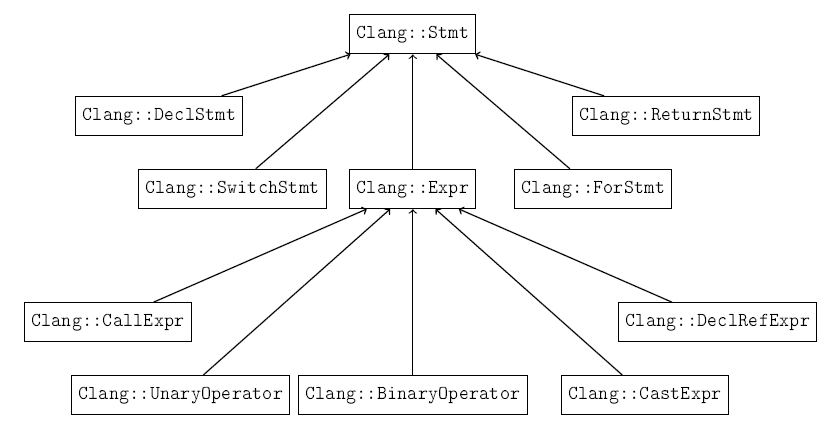
\includegraphics[scale=0.7]{soluce/graph.jpg} 
 %      \caption{Partie de l'architecture de Clang}
  %     \label{fig:graph}
  %   \end{figure}
